\documentclass[]{article}

\usepackage{caption}
\usepackage{subcaption}
\usepackage{graphicx}
\usepackage{float}
\usepackage{url}
\usepackage{amsmath}
\usepackage{amssymb}
\usepackage{amsthm}
\usepackage{tocloft}
\usepackage{cancel}
\usepackage{thmtools}
\usepackage{gensymb}
\usepackage{braket}
\usepackage{tikz-feynman}
\usepackage{tikz}
\usepackage{mathtools}
\usepackage{color}
\usepackage{colortbl}
\usepackage[toc,nonumberlist]{glossaries}
\usepackage{glossaries-extra}
\usepackage[T1]{fontenc}
\usepackage[utf8]{inputenc}
\usepackage[toc,page]{appendix}
\newcommand\numberthis{\addtocounter{equation}{1}\tag{\theequation}}
\newcommand{\Lagr}{\mathscr{L}}
\newtheorem{thm}{Theorem}
\newtheorem{defn}[thm]{Definition}
\newtheorem{cor}[thm]{Corollary}
\newtheorem{lemma}[thm]{Lemma}
\graphicspath{{figs/}}
\widowpenalty10000
\clubpenalty10000
\setcounter{tocdepth}{2}

%opening
\title{Theoretical Minimum\\Cosmology}
\author{Simon Crase (compiler)\\simon@greenweaves.nz}

\makeglossaries

\begin{document}

\maketitle

\begin{abstract}
	These are my notes for the \emph{Cosmology}\cite{susskind2013cosmology} lectures from Leonard Susskind's \emph{Theoretical Minimum} series\cite{susskind2007theoretical}. 
	
	Disclaimer: I have created these notes as an aide-m\'emoire for my own use; if you find them useful, you are welcome, but I'd appreciate hearing from you. They are not intended as a substitute for listening to the lectures. The intellectual property for all material derived from the lectures belongs, of course, to Professor Susskind; any mistakes, however, are my own.
	
	The notes were created using TexStudio\cite{TexStudio}, and the bibliography using JabRef\cite{Jabref}.
\end{abstract}

\tableofcontents
\listoffigures
\listoftables
\listoftheorems

\newglossaryentry{gls:isotropic}{
	name={isotropic},
	description={In physics and geometry, isotropy  is uniformity in all orientations--\cite{enwiki:1230543452}}}

\newglossaryentry{gls:homogenous}{
	name={homogenous},
	description={Homogeneity means the space is every where the same. Somebody located at a particular place in the space looks around them, see everywhere around them, and sees exactly the same thing that somebody else sees in any other position\cite[Lecture 3]{susskind2013cosmology}}}	
\newglossaryentry{gls:scale:factor}{
	name={scale factor},
	description={The expansion of the universe is parametrized by a dimensionless scale factor $a$.  It relates the proper distance (which can change over time, unlike the comoving distance $d_C$ which is constant and set to today's distance) between a pair of objects, e.g. two galaxy clusters, moving with the Hubble flow in an expanding or contracting FLRW universe at any arbitrary time $t$ to their distance at some reference time $t_0$.\cite{enwiki:1228037646}}}

\newglossaryentry{gls:peculiar:velocity}{
	name={peculiar velocity},
	description={The components of a galaxy's velocity that deviate from the Hubble flow. According to Hubble's Law, galaxies recede from us at speeds proportional to their distance from us.\cite{enwiki:1192597030}}}
			
\section{The expanding (Newtonian) universe}\label{sec:expanding:newton}

\begin{quotation}
	This lecture focuses on the classical or Newtonian view of the universe.  Beginning with the assumption of an isotropic universe with gravity as the only significant cosmic-scale force, Professor Susskind derives the equation for the Hubble constant, and demonstrates that the universe cannot be static -- that it must be expanding or contracting.
\end{quotation}

Cosmology as a science dates back to the discovery of the microwave radiation from the Big Bang in the 1960s. Before that Cosmology was more like natural science--classifying oddities. Thinking of the universe as a physical system, as a system to study mathematically, with a set of physical principles and a set of equations, is relatively new.

We will study the universe as a physical system, i.e. something we can study with equations.

\begin{itemize}
	\item First observation: the universe is \gls{gls:isotropic}, averaging over patches of the sky, so it should be \gls{gls:homogenous}. If not we'd have shells centered on Earth!

	\item There are around $10^{11}$ galaxies within view of Earth, which we can treat as particles. Each galaxy has roughly $10^{11}$ stars.
	
	\item Gravity is the only force that matters at cosmological scales: it pulls stuff together. Should stuff remain static?
\end{itemize}

Could Newton have figured out expanding universe given observations?

\subsection{How would Newton have handled expanding universe?}

\begin{figure}[H]
	\begin{center}
		\caption{We start by introducing a set of coordinates.}
		\begin{subfigure}[b]{0.4\textwidth}
			\caption{Chose grid so that galaxies are at grid points, so grid moves with galaxies. Galaxies move coherently (from observation).}\label{fig:cosmo-1-grid}
			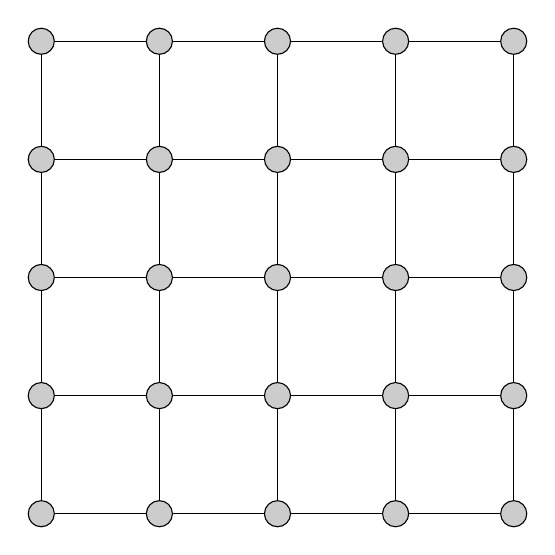
\begin{tikzpicture}[darkstyle/.style={circle,draw,fill=gray!40,minimum size=1}]
				\foreach \x in {0,...,4}
				\foreach \y in {0,...,4} 
				{\pgfmathtruncatemacro{\label}{\x - 5 *  \y +21}
					\node [darkstyle]  (\x\y) at (1.5*\x,1.5*\y) {};} 
				
				\foreach \x in {0,...,4}
				\foreach \y [count=\yi] in {0,...,3}  
				\draw (\x\y)--(\x\yi) (\y\x)--(\yi\x) ;
				
			\end{tikzpicture}
		\end{subfigure}
		\hfill
		\begin{subfigure}[b]{0.4\textwidth}
			\caption{Define distance: $D_{ab}=a(t) \Delta x_{ab}$, where \gls{gls:scale:factor} $a$ may or may not be a constant.}\label{fig:cosmo-1-distance}
			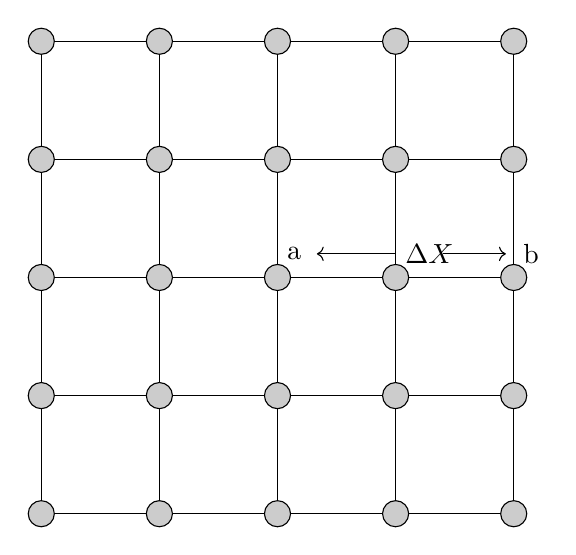
\begin{tikzpicture}[darkstyle/.style={circle,draw,fill=gray!40,minimum size=1}]
				\foreach \x in {0,...,4}
				\foreach \y in {0,...,4} 
				{\pgfmathtruncatemacro{\label}{\x - 5 *  \y +21}
					\node [darkstyle]  (\x\y) at (1.5*\x,1.5*\y) {};} 
				
				\filldraw[black] (1.5*2,1.5*2+0.3) node[anchor=west]{a}; 
				\filldraw[black] (1.5*4,1.5*2+0.3) node[anchor=west]{b}; 
				\filldraw[black] (1.5*3,1.5*2+0.3) node[anchor=west]{$\Delta X$}; 
				\draw[->]        (1.5*3+0.6,1.5*2+0.3)   -- (1.5*4-0.1,1.5*2+0.3);
				\draw[->]        (1.5*4-1.5,1.5*2+0.3)   -- (1.5*2+0.5,1.5*2+0.3);
				\foreach \x in {0,...,4}
				\foreach \y [count=\yi] in {0,...,3}  
				\draw (\x\y)--(\x\yi) (\y\x)--(\yi\x) ;
				
			\end{tikzpicture}
		\end{subfigure}
	\end{center}
\end{figure}
 
 We postulate a more general formula for distance between two galaxies $a$ and $b$:
 
 \begin{align*}            
 	D_{ab}=&a(t) \sqrt{\Delta_{ab} x^2 + \Delta_{ab} y^2 + \Delta_{ab} z^2}  \text{, where $a(t)$ is called the ''scale factor''}
\end{align*}
 Now calculate velocity:\footnote{\label{note1}During the lecture, $V$ is used for both velocity and volume. I will retain this usage in the notes; the reader should be careful to check which usage is meant.}           
 \begin{align*}	
 	V_{ab}=&\dot{a} \Delta X_{ab} \text{, neglecting $y$ and $z$}\\
 	\frac{V_{ab}}{D_{ab}} =& \frac{\dot{a}}{a} \text{, independent of choice of galaxies!}\\
 	=& H \text{, Hubble constant at a given time.}\\
 	V =& H D \text{, Hubble's Law.}
\end{align*}
 
\subsection{How much mass is in $\Delta x \Delta y \Delta z$?}

Assume  $\Delta x \Delta y \Delta z$ big enough that we can average over the small scale structure. How much mass is in there? Let $M$ denote the mass within $\Delta x \Delta y \Delta z$, and $M = \nu \Delta x \Delta y \Delta z$. Let $V$ denote the volume\textsuperscript{\ref{note1}}.

\begin{align*}
	V =& a^3 \Delta x \Delta y \Delta z\\
	M =& \nu \Delta x \Delta y \Delta z \text{, constant}\\
	\rho(t) =& \frac{\nu}{a(t)^3} \numberthis \label{eq:rho}
\end{align*}

Amount of mass in a given region of Figure \ref{fig:cosmo-1-grid} remains the same, as galaxies move with grid.

\subsection{Newtonian derivation of Friedmann's equation}
Choose grid so Newton is at rest at centre of universe. He looks out at distant galaxy, which moves in accordance with Newton's laws. He would use Newton's Theorem--Figure \ref{fig:newtons:thm} and Theorem \ref{thm:newton:shell}.

\begin{thm}[Newton's shell theorem]\label{thm:newton:shell}
	\begin{enumerate}
		\item A spherically symmetric body affects external objects gravitationally as though all of its mass were concentrated at a point at its center.
		\item If the body is a spherically symmetric shell (i.e., a hollow ball), no net gravitational force is exerted by the shell on any object inside, regardless of the object's location within the shell.
	\end{enumerate}
\end{thm}

\begin{proof}
	Given in \cite{enwiki:1241447151}.
\end{proof}

\begin{figure}[H]
	\caption[Newton's Theorem]{Newton's Theorem: to determine gravitational force on red body, assuming isotropy, draw sphere and calculate force as if mass inside shell were concentrated in centre, and ignore mass outside.}\label{fig:newtons:thm}
	\begin{center}
		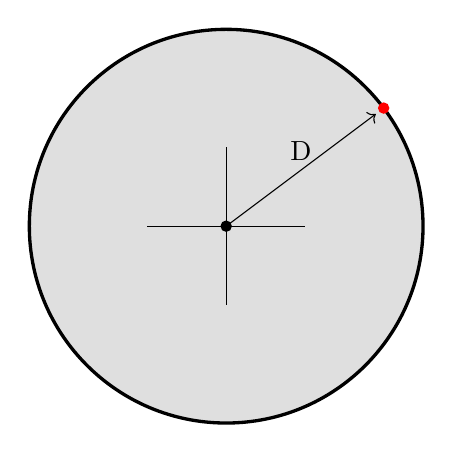
\begin{tikzpicture}[scale=0.5]
			\filldraw[color=black, fill=gray!25, very thick](0,0) circle (5.0);
			\filldraw[color=red, fill=red, very thick](4,3) circle (0.1);
			\filldraw[color=black, fill=black, very thick](0,0) circle (0.1);
			\draw[black] (-2,0) -- (2,0);
			\draw[black] (0,-2) -- (0,2);
			\draw[black,->] (0,0) -- (4*0.95,3*0.95) node[midway, above] {D};
		\end{tikzpicture}
	\end{center}
\end{figure}

\begin{align*}
	D =& a(t) \sqrt{x^2 + y^2 + z^2}\\
	=&a(t) R \text{, say} \numberthis \label{eq:D}
\end{align*}
R is constant, since galaxy is located at a fixed point in lattice. We want acceleration so we can use Newton's laws.
\begin{align*}
	V =& \dot{a(t)} R\\
	A =& \ddot{a(t)}R
\end{align*}
From Newton's Law of Universal Gravitation
\begin{align*}
	F =& - \frac{mMG}{D^2}\\
	A =& - \frac{MG}{D^2} \text{, which should become}\\
	=& \ddot{a(t)}R
\end{align*}
So we want
\begin{align*}
	\ddot{a(t)}R =& - \frac{MG}{D^2}\\
	=& - \frac{MG}{a^2 R^2} \text {, from \eqref{eq:D}}\\
	\frac{\ddot{a(t)}}{a} =& - \frac{MG}{a^3 R^3}\text{, now volume is}\\
	V =& \frac{4 \pi}{3}  a^3 R^3\\
	\frac{\ddot{a(t)}}{a}=& -\frac{4 \pi}{3} G \rho \text{, from definition of $\rho$} \numberthis \label{eq:a}
\end{align*}

Now $\rho$ does not depend in $R$, so \eqref{eq:a} applies for every galaxy. This is true for any origin, as long as we do the transformation carefully. Everything hinges on the assumption that the universe is homogeneous.

We can see from \eqref{eq:a} that the universe is not static unless $\rho=0$. Let us substitute \eqref{eq:rho} in \eqref{eq:a}.

\begin{align*}
	\frac{\ddot{a(t)}}{a} =& -\frac{4 \pi}{3} \frac{G \nu}{a^3}  \numberthis \label{eq:friedmann}
\end{align*}

This was discovered by Friedmann, in the context of General Relativity. It doesn't tell us whether universe is expanding or contracting, but tells us that acceleration is negative. But observation says that it isn't! This would have been the standard model before we found that expansion is accelerating.

\begin{figure}[H]
	\caption{Consider throwing rock up from Earth, along x-axis}\label{fig:cosmo:throw:rock}
	\begin{center}
		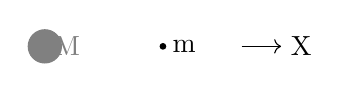
\begin{tikzpicture}[scale=0.5]
			\filldraw[gray] (0,0) circle (12pt) node[anchor=west]{M};
			\filldraw[black] (3,0) circle (2pt) node[anchor=west]{m};
			\draw [->] (5,0)   -- (6,0) node[right] {X};
		\end{tikzpicture}
	\end{center}
\end{figure}

We will write down the energy equation: total energy is $\frac{1}{2}m v^2 -\frac{m M G}{x}$. What is escape velocity if total energy is zero?
\begin{align*}
	\frac{1}{2}\cancel{m} V^2 -\frac{\cancel{m} M G}{X} =& 0\\
	V^2 =& \frac{2 M G}{X}
\end{align*}
Similarly in \eqref{eq:friedmann}, total energy can by positive, negative or zero.
\begin{itemize}
	\item If energy great enough, universe does not turn around: it expands forever.
	\item If energy smaller, universe eventually contracts.
	\item Escape velocity is the boundary between the other two cases.
\end{itemize}

In Figure \ref{fig:newtons:thm}, all the particle knows is that it is moving under influence of mass concentrated at origin, so we can treat as Figure \ref{fig:cosmo:throw:rock}.

The Total Energy is given by $\frac{1}{2} m \dot{a}^2 R^2 -\frac{m M G}{a R}$. In the edge case where energy is zero:
\begin{align*}
	 \dot{a}^2 R^2 -\frac{2 M G}{a R} =& 0 \\
	 \frac{\dot{a}^2 }{a^2} -\frac{2 M G \frac{4}{3} \pi}{\frac{4}{3} \pi a^3 R^3} =& 0 \\
	 {\underbrace{\big(\frac{\dot{a}}{a}\big)}_\text{Hubble}}^2 =& \frac{8 \pi}{3} G \rho \numberthis \label{eq:friedmann:eq}
\end{align*}
Equation \eqref{eq:friedmann:eq} is known as the Friedmann equation. This universe will get slower and slower, but never collapse.

Using \eqref{eq:rho}, \eqref{eq:friedmann:eq} becomes:
\begin{align*}
	\big(\frac{\dot{a}}{a}\big)^2 =& \frac{8 \pi \nu}{3}\frac{G}{a^3} \numberthis \label{eq:friedmann:8} \text{, or, using suitable units}\\
	\big(\frac{\dot{a}}{a}\big)^2 =& \frac{1}{a^3} \numberthis \label{eq:friedmann:8a}
\end{align*}
The right hand side of \eqref{eq:friedmann:8a} is always positive, and decreases as $a$ increases, but slows. We will attempt a trial solution, putting $a=ct^P$.
\begin{align*}
	a=&ct^P\\
	\dot{a}=&c P t^{P-1}\\
	\frac{\dot{a}}{a}=& \frac{P}{t} \text{. so \eqref{eq:friedmann:8a} becomes:}\\
	\frac{P^2}{t^2} =& \frac{1}{c^3 t^{3P}} \text{, whence}\\
	3P =& 2\\
	P =& \frac{2}{3}\\
	P^2 =& \frac{1}{C^3}
\end{align*}

\begin{figure}[H]
	\caption[Scale Factor]{Scale Factor, showing slowing (case discusses), collapsing, and real (accelerating) universes.}
	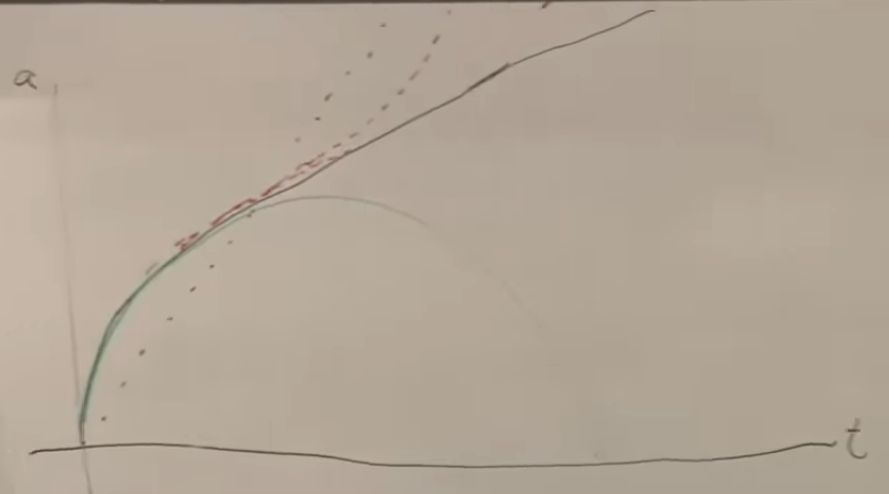
\includegraphics[width=\textwidth]{cosmo-1-scale-factor}
\end{figure}

Newton speculated about a homogeneous universe, but didn't carry out the calculation.

\section{Matter and radiation dominated universes}\label{sec:matter:radiation:dominated}

\begin{quotation}
	After reviewing the basic equation for an expanding universe, Professor Susskind solves the equation explicitly for a zero energy universe, and then extends the derivation to universes with non-zero energy.  These universes can take two forms: matter-dominated universes, and radiation-dominated universes.  The radiation-dominated form characterizes our early universe, and the matter-dominated form characterizes our universe today -- or so cosmologists believed until observations led to theories of dark energy in the 1990s.
\end{quotation}

Did Newton get it right? Yes, mostly. Einstein's equations deal with curved space-time, and some of the universes we will study have curved 3-space, maybe a 3-sphere. Suppose we just look at very neighbouring galaxies, where it will look flat. Then in a small region we can use Newton;s equations. So what we did in Section \ref{sec:expanding:newton} should be OK, as long as we don't have two galaxies moving past each other at a speed comparable to that of light (But that is OK for galaxies that are a long way away).

Now photons and neutrinos are moving very fast, so  we have to modify our equations to deal with this.

Treat matter in galaxies as uniform density $\rho$. Lay down grid as in Figure \ref{fig:cosmo-1-grid}. How big is spacing? Equations should not depend on spacing, but maybe the ratios matter. If $a$ doubles, we have expansion.
\begin{figure}[H]
	\caption{Equations should not depend on spacing.}
	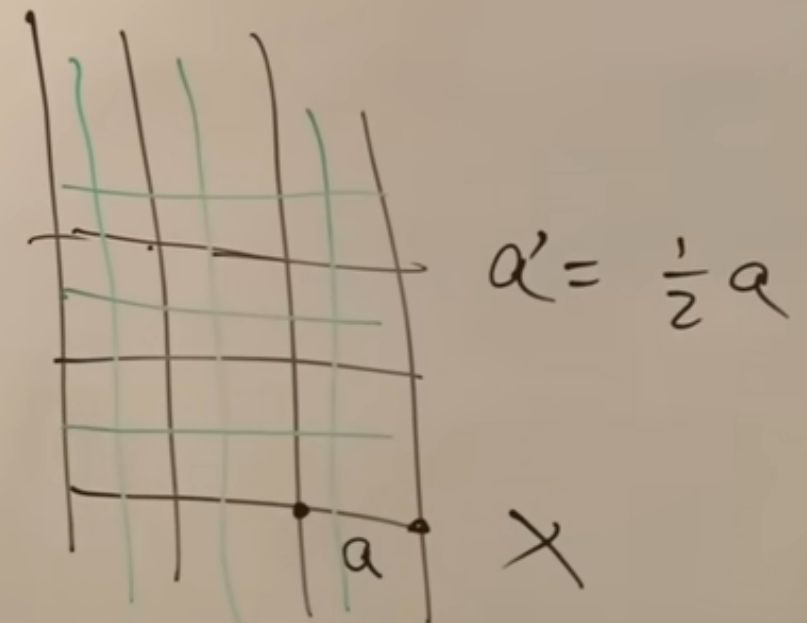
\includegraphics[width=0.8\textwidth]{cosmo-2-grid}
\end{figure}

We could measure expansion by $\frac{\dot{a}}{a}$.

Another ambiguity is $\nu$, which depends on $a$.

In Section \ref{sec:expanding:newton} we derived \eqref{eq:friedmann:8}, which reduces to:
\begin{align*}
	\big(\frac{\dot{a}}{a}\big)^2 =& \frac{8 \pi G \rho}{3}
\end{align*}

$\frac{8 \pi}{3}$ is related to the volume of a sphere. The equation assumes zero energy, or, equivalently, galaxies moving at escape velocity.

Is $\nu$ constant? If we assume, for the moment, that protons and galaxies are forever, then yes, $\nu$ is constant. Box grows, but number of particles in box remains constant. Recall \eqref{eq:friedmann:8}:
\begin{align*}
	\big(\frac{\dot{a}}{a}\big)^2 =& \frac{8 \pi \nu}{3}\frac{G}{a^3} \\
	\big(\frac{\dot{a}}{a}\big)^2 =& \frac{1}{a^3} \text{, using suitable units} \numberthis \label{eq:friedmann:normalized}
\end{align*}

We can solve \eqref{eq:friedmann:normalized}.

\begin{align*}
	\dot{a} =& \frac{1}{\sqrt{a}}\\
	\frac{dt}{da} =& \sqrt{a} \text{, $\pm$ corresponds to expansion/contraction} \\
	t = \frac{2}{3}a^{\frac{3}{2}}\\
	a = t^\frac{2}{3} \text{, ignoring some constant} \numberthis \label{eq:2:3}
\end{align*}

\begin{figure}
	\caption[Decelerating growth of scale parameter]{Scale parameter increases with time, but decelerates as the result of gravitational attraction}
	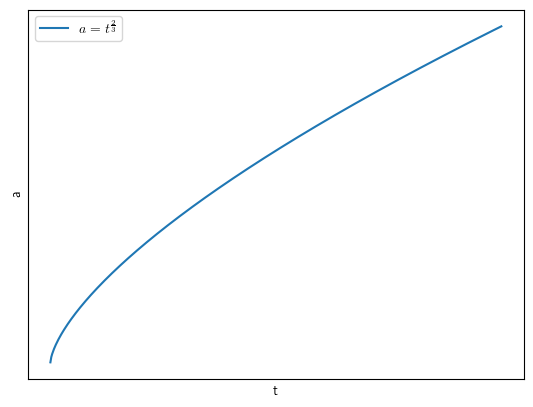
\includegraphics[width=0.8\textwidth]{figs/cosmo-2-a-t}
\end{figure}


	
NB. Real motion of galaxies is made up of flow plus \gls{gls:peculiar:velocity}.

There are two directions we want to go in.
\begin{enumerate}
	\item What if we replace matter with photons? (Early universe). Section \ref{sec:radiation:dominated}
	\item What if energy is non-zero?--Section \ref{sec:matter:dominated}.
\end{enumerate}

\subsection{Matter dominated universe}\label{sec:matter:dominated}
\begin{figure}[H]
	\caption{We compute the constant energy}
		\begin{center}
			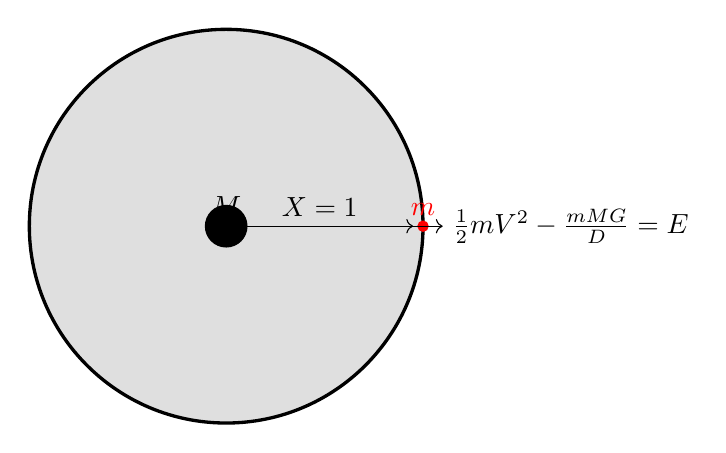
\begin{tikzpicture}[scale=0.5]
				\filldraw[color=black, fill=gray!25, very thick](0,0) circle (5.0);
				\filldraw[color=red, fill=red, very thick](5,0) circle (0.1) node[right,above]{$m$};
				\filldraw[color=black, fill=black, very thick](0,0) circle (0.5) node[above]{$M$};
				\draw[black,->] (0,0) -- (5*0.95,0) node[midway, above] {$X=1$};
				\draw[black,->] (5*0.95,0) -- (5.5,0) node[right] {$\frac{1}{2}m V^2 - \frac{mMG}{D}=E$};
			\end{tikzpicture}
	\end{center}
\end{figure}

\begin{align*}
	 V^2 -  \frac{2MG}{D} =& \frac{2E}{m}\\
	 D =& aX \\
	 V =& \dot{a} X \text{, but we have set $X=1$}\\
	 D =& a \\
	 V =& \dot{a} \text{, so the energy equation becomes}\\
	 \dot{a}^2 - \frac{2MG}{a} =& C \text{, say}\\
	 \big(\frac{\dot{a}}{a}\big)^2 - \frac{2MG}{a^3} =& \frac{C}{a^2} \\
	 \big(\frac{\dot{a}}{a}\big)^2 - \frac{8\pi\rho G}{3} =& \frac{C}{a^2}\\
	 \big(\frac{\dot{a}}{a}\big)^2  =& \frac{8\pi\nu G}{3a^3} + \frac{C}{a^2} \text{, on substituting \eqref{eq:rho}} \numberthis \label{eq:full:friedmann}
\end{align*}

Equation \eqref{eq:full:friedmann} is the full Friedmann equation, which he derived from General Relativity; we have derived from Newton.

if $C>0$, right hand side is strictly positive, universe continues to grow forever (For if $\dot{a}>0$ initially, it has to pass through zero to stop expanding). If $a$ small enough $\frac{8\pi\nu G}{3 a^3}$ will dominate, and we can use \eqref{eq:2:3}. Once $a$ grows enough $ \frac{C}{a^2}$ dominates.

\begin{align*}
	\big(\frac{\dot{a}}{a}\big)^2  =&  \frac{C}{a^2} \\
	\frac{\dot{a}}{a} =&  \frac{C}{a} \text{, for some new $C$}\\
	\dot{a} =& C
\end{align*}

Eventually we can neglect gravity and velocity is uniform.

What if energy is negative? Equation \eqref{eq:full:friedmann} becomes:

\begin{align*}
	\big(\frac{\dot{a}}{a}\big)^2  =& \frac{8\pi\nu G}{a^3} - \frac{C}{a^2} \text{, for some new, positive $C$}
\end{align*}
Now there is a point where $\dot{a}=0$: the expansion stops, and $\dot{a}$ changes from positive branch of square root to negative.

\begin{figure}[H]
	\caption{Negative Energy:  there is a point where $\dot{a}=0$}
	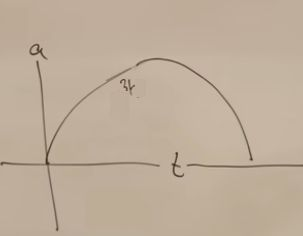
\includegraphics[width=0.8\textwidth]{cosmo-2-negative}
\end{figure}

The matter dominated universe was the classic cosmology until other things were discovered. There are three cases, positive energy, negative and zero. In a later lecture we will find that this is connected to the geometry of the universe: this is the main contribution of General Relativity.


\subsection{Radiation dominated universe}\label{sec:radiation:dominated}

We do have to think about relativity, but there is only one important thing: $E=mc^2$. We rewrite Equation \eqref{eq:full:friedmann} to show the connection with general relativity, and define $\kappa = C$:

\begin{align*}
	\underbrace{\big(\frac{\dot{a}}{a}\big)^2  - \frac{\kappa}{a^2}}_\text{Terms involving geometry}=& \underbrace{\frac{8\pi}{3} G \rho}_\text{Matter and energy} \numberthis \label{eq:geometry:energy}
\end{align*}
We'll replace mass density with energy density. Energy = $Mc^2 + $ Radiation (and we will choose units such that $c=1$).

To compute radiation density, take a box, volume $a^3$, and assume a certain number of photons.

\begin{figure}[H]
	\caption{Unit box with photons: $\lambda$ increases as box expands adiabatically }\label{fig:unit:box}
	\begin{center}
			\begin{subfigure}[t]{0.45\textwidth}
				\begin{center}
					\caption{As box expands adiabatically, photons do work on walls of box. Number of photons does not change.}
					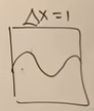
\includegraphics[width=\textwidth]{cosmo-2-unit-box}
				\end{center}
			\end{subfigure}
			\;
			\begin{subfigure}[t]{0.45\textwidth}
				\begin{center}
					\caption{An analogy with standing waves. Number of nodes (zero crossings) is an adiabatic invariant:  it has to be an integer. So $\lambda$ stretches with circle.}
					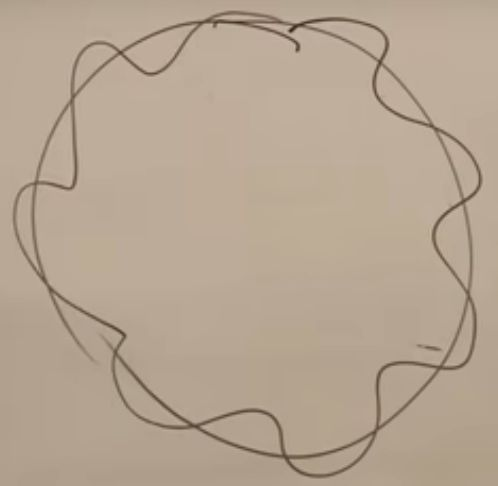
\includegraphics[width=\textwidth]{cosmo-2-standing-waves}
				\end{center}
			\end{subfigure}	
	\end{center}
\end{figure}

\begin{align*}
	V =& a^3\\
	E =& \frac{h c}{\lambda}
\end{align*}

We have to do some more quantum mechanics of classical electromagnetism to justify the statement in Figure \ref{fig:unit:box}. For the time being, take it as a given. So energy in box decreases: $E\propto \frac{1}{a}$ and $\rho\propto \frac{1}{a^4}$. We substitute in \eqref{eq:geometry:energy}:

\begin{align*}
	\big(\frac{\dot{a}}{a}\big)  =& \frac{8\pi\nu G}{a^4} - \frac{C}{a^2} \text{, and explore the case where $C=0$}\\
	\big(\frac{\dot{a}}{a}\big)  =& \frac{8\pi\nu G}{a^4} \text{, or, with suitable units}\\
	\big(\frac{\dot{a}}{a}\big)  =& \frac{1}{a^4} \text{, taking square root and rearranging} \\
	\dot{a} =& \frac{1}{a}\\
	\frac{dt}{da} =& a\\
	t =& a^2 \text{, in suitable units}\\
	a =& \sqrt{t} \numberthis \label{eq:a:scrt:t}
\end{align*}

\begin{figure}[H]
	\caption[Comparison of radiation and matter dominated universes]{Comparison of radiation and matter dominated universes--\eqref{eq:2:3} and \eqref{eq:a:scrt:t}}\label{fig:cosmo-2-a-r}
	\begin{center}
			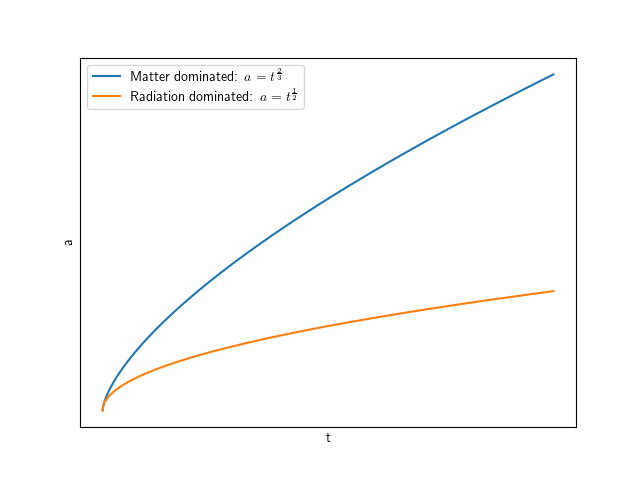
\includegraphics[width=0.8\textwidth]{cosmo-2-a-r}
	\end{center}
\end{figure}


\subsection{Mixed case: neither matter nor radiation dominates}

We consider a real universe with both matter and radiation.

\begin{align*}
	\big(\frac{\dot{a}}{a}\big)^2 =& \underbrace{\frac{C_m}{a^3}}_\text{More important for big $a$} + \underbrace{\frac{C_R}{a^4}}_\text{More important for small $a$}
\end{align*}

At start of expansion, radiation dominates, $t^{\frac{1}{2}}$, but later switches, $t^{\frac{2}{3}}$--Figure \ref{fig:cosmo-2-a-r}.

\begin{itemize}
	\item How do we know that there isn't conversion of matter to energy as universe expands? In practice mostly conserved separately once things cool to 1000K.

	\item There is a third component: dark energy (dark matter is included in $C_m$).

	\item Radiation includes photons, gravitons, and neutrinos, which move at speeds close to $c$.
\end{itemize}

This is the cosmology of 30 years prior to date of lecture (2013).

What happens to radiation energy lost during expansion?
\begin{align*}
	\underbrace{- \big(\frac{\dot{a}}{a}\big)^2}_\text{Kinetic Energy} + \frac{C_m}{a^3} +\frac{C_R}{a^4} =& 0 
\end{align*}

Kinetic Energy is  tiny at present.

There are two ways to think about time translation symmetry.
\begin{enumerate}
	\item The universe is a time dependent thing that everything moves in. There is no longer time translation symmetry, so energy doesn't have to be conserved.
	\item There is time translation symmetry: starting universe at $t=-7$ is exactly that same as starting at $t=4$, but this adds an extra term to energy equation. This is very subtle and we'll discuss later.
\end{enumerate}

There are three cases in \eqref{eq:geometry:energy}.

\begin{align*}
	\big(\frac{\dot{a}}{a}\big)^2  =& \frac{8\pi\rho G}{3} - \frac{\kappa}{a^2} 
\end{align*}

In Section \ref{sec:geometries}, we will see that $\kappa$ is connected with geometry.
\begin{itemize}
	\item If $\kappa=0$, space is flat.
	\item If $\kappa>0$, space is curved like a sphere, and it compact.
	\item If $\kappa<0$, space is curved negatively.
\end{itemize}


\section{Geometries of space: flat, spherical, hyperbolic} \label{sec:geometries}

\begin{quotation}
	Professor Susskind presents three possible geometries of homogeneous space: flat (infinite), spherical (positively curved and finite), hyperbolic (negatively curved and infinite). He develops the metric for these three spatial geometries in spherical coordinates, and describes methodologies for determining which geometry represents our universe. To date, we have not been able to detect curvature in our universe. Professor Susskind concludes the lecture by introducing a time-dependent scale factor into the metric for each of these geometries.
\end{quotation}

As a matter of observation, space \emph{is} flat. We don't know that it is flat, just that it is very big, and we don't know whether there is any curvature. It is important to investigate the various possibilities. We don't know what is happening on scales beyond 10 billion light years, but we will make some assumptions. We won't assume that it is flat, but we will assume that it is homogeneous and isotropic. Is that true? We don't know, but we can only test it if we know its consequences. Almost all cosmology is based on that assumption.

If space is not flat, it must be curved. While there are many types of curved spaces, most are not compatible with the universe being \gls{gls:homogenous}.

\begin{itemize}
	\item A parabaloid is most certainly not homogeneous. Its curvature is greater at the tip, less further away.
	\item A long pointy ellipsoid is not homogeneous. You would notice the difference if you were walking around on it.
	\item Surfaces with bumps are not homogeneous.
\end{itemize}

What kinds of spaces \emph{can} be curved and homogeneous? There are two kinds, positive curvature, Section \ref{sec:positive:curvature}, and negative, Section \ref{sec:negative:curvature}.

\subsection{Flat Space and the 3-sphere}\label{sec:positive:curvature}

Let's think about a metric for ordinary flat space, restricting to 2 dimensions.

\begin{align*}
	ds^2 =& dx^2 + dy^2\text{, or changing to polar coordinates}\\
	=&dr^2 + r^2 d\theta^2 \text{, or changing notation}\\
	=&dr^2 + r^2 d\Omega_1^2 \numberthis \label{eq:flat:polar}
\end{align*}

Use the idea that $d\theta^2$ is a  metric for $\Omega_1$, the 1-sphere or unit circle.

\begin{figure}[H]
	\caption[We can treat a circle as a piece of string and deform it]{We can treat circle as a piece of string and deform it. Label by angular coordinate so equal distances map to the equal angles. A circle is just a curve where we come back to the same place after an angle of $2\pi$.}
	\begin{center}
		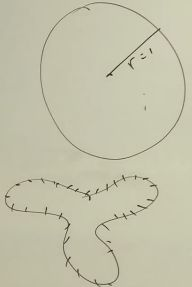
\includegraphics[width=0.8\textwidth]{cosmo-3-1-sphere}\label{fig:cosmo-3-1-sphere}
	\end{center}
\end{figure}

In polar coordinates, it \emph{looks} as if there is a special place, but, in reality, all points are the same. We will think of flat 2d space as a nested collection of circles--\eqref{eq:flat:polar}. 

The 2-sphere is also homogeneous. Every point on the surface of the sphere is the same as any other point. It has uniform curvature. If you walk around you come back to the same space.

\begin{figure}[H]
	\caption[Nested spheres with point indicating observer]{Nested spheres with point indicating observer. Observer looks out and sees a series of nested spheres, maybe one light year apart. They start growing, slow down, and then contract. Characterize spheres by angle $r$. We will denote the 2-sphere $\Omega_2$.} 
	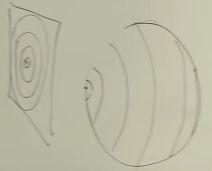
\includegraphics[width=0.8\textwidth]{cosmo-3-1-nested-spheres}
\end{figure}

The metric of the 2-sphere is:

\begin{align*}
	d\Omega_2^2 =& dr^2 + \sin^2 r\; d\Omega_1^2
\end{align*}

This pattern just continues. If I want to make a 3 dimensional sphere--a 3 dimensional space where every point is the same, and where we eventually come back to the same point. If we look into space for a certain distance, things form a 2-sphere. Look further, a bigger 2-sphere, but eventually they start to get smaller.

\begin{figure}[H]
	\caption[Nested 2-spheres in a 3-sphere]{Nested 2-spheres in a 3-sphere. The observer is in the 3-sphere, at the point $r=0$. The 2-spheres surround the observer.}
	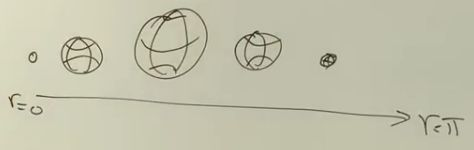
\includegraphics[width=0.8\textwidth]{cosmo-3-3-sphere}
\end{figure}

The metric follows the familiar pattern:
\begin{align*}
	d\Omega_3^2 =& dr^2 + \sin^2 r\; d\Omega_2^2
\end{align*}

What happens in flat space? In polar coordinates, \eqref{eq:flat:polar} generalizes to:
\begin{align*}
	ds^2 =& dr^2 + r^2 d\Omega_2^2
\end{align*}

There is another way to view spheres. Imagine an ant living on a circle. It can receive light along the circle, it can communicate with its neighbours, but it has no way of knowing whether it lives on either curve in Figure \ref{fig:cosmo-3-1-sphere}, or even whether there are additional dimensions. We, however, can describe a circle by embedding it in two dimensions.
\begin{figure}[H]
	\caption{Embedding an $n$-sphere in $n+1$ dimensions}
	\begin{subfigure}[t]{0.5\textwidth}
		\caption{A circle in two dimensions: $x^2 + y^2 = 1$}
		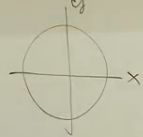
\includegraphics[width=0.8\textwidth]{cosmo-3-embed-circle}
	\end{subfigure}
	\begin{subfigure}[t]{0.5\textwidth}
		\caption{A 2-sphere in three dimensions: $x^2 + y^2 + z^2= 1$}
		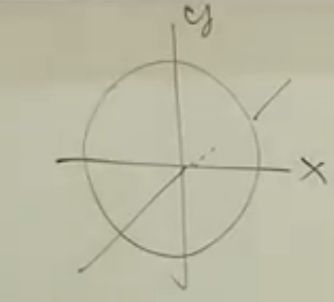
\includegraphics[width=0.8\textwidth]{cosmo-3-embed-2-sphere}
	\end{subfigure}
\end{figure}
Similarly we can embed a 3-sphere in 4 dimensions: $x^2 + y^2 + z^2+w^2= 1$. We don't have to answer the question whether this makes physical sense.


What is the difference in what we perceive between a sphere and an infinite flat plane? Suppose we had telescopes that allow us to determine the distance to distant objects. The telescope doesn't measure $r$, but there are tricks, e.g. spectroscopy, brightness(assume galaxies the same). We ask what angle they subtend. 

\begin{figure}[H]
	\caption{Standard Galaxies in flat space}
	\begin{subfigure}[t]{0.45\textwidth}
		\caption{Standard galaxy has width $d$}
		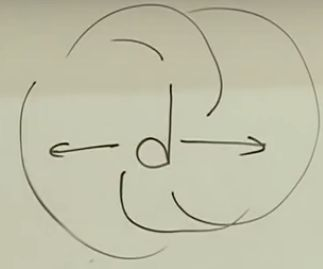
\includegraphics[width=\textwidth]{cosmo-3-3-standard-galaxy}
	\end{subfigure}
	\begin{subfigure}[t]{0.45\textwidth}
		\caption{For flat space, the observer perceives the width of the galaxy to be $ds^2 = r^2$, so $d\theta^2 = d^2$}
		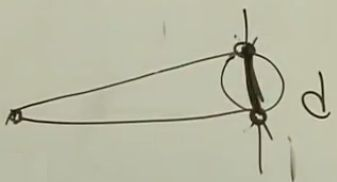
\includegraphics[width=\textwidth]{cosmo-3-3-standard-galaxy-flat-space}
	\end{subfigure}
\end{figure}

Now, consider the 2-sphere.

\begin{figure}[H]
	\caption{Galaxies embedded in 2-sphere, with observer at "left pole".}
	\begin{center}
		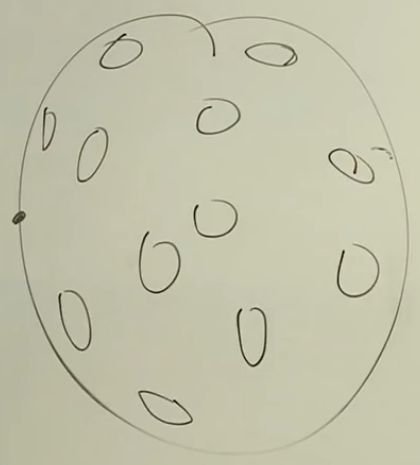
\includegraphics[width=0.6\textwidth]{cosmo-3-galaxies-2-sphere}
	\end{center}
\end{figure}

\begin{align*}
	d^2 =& \sin^2 r d\theta^2\\
	d\theta =& \frac{d}{\sin r}
\end{align*}

$d\theta$ is bigger than if we lived in flat space. Distant galaxies appear bigger, but fainter. So we can distinguish flat and spherical.

We can also count the number of galaxies: on  a sphere you see fewer galaxies at great distances, compared to the plane. At antipodes we see just one galaxy.

\begin{figure}[H]
	\caption[Stereographic Projection]{Stereographic Projection: observer is at South pole. Every point on sphere projects to a point on plane, and North pole projects to infinity. Circles on sphere map to little closed curves on plane (actually circles).}
	\begin{center}
			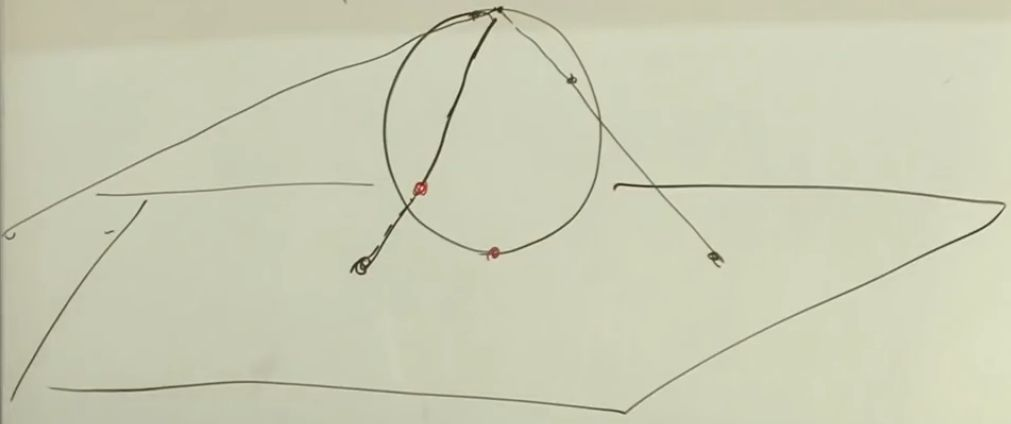
\includegraphics[width=0.6\textwidth]{cosmo-3-stereographic-projection}
	\end{center}
\end{figure}

How do circles on the plane map to circles on the sphere? If they are close to South pole they look the same. As we move further the projections get bigger, and the extreme Arctic circle looks very large. Sphere is homogeneous, but this doesn't match plane. 

We can do the same thing with a 3-sphere.

\subsection{Hyperbolic geometry}\label{sec:negative:curvature}
There is a third homogeneous geometry, which we'll call the hyperbolic space. As we move from observer, size of circles blows up very rapidly.

\begin{align*}
	d\mathcal{H}_2^2 =& dr^2 + \sinh^2 r d\Omega_1^2\\
	d\mathcal{H}_3^2 =& dr^2 + \sinh^2 r d\Omega_2^2 \text{, candidate geometry for our space.}
\end{align*}

What happens to angle subtended by a galaxy?

\begin{align*}
	d\theta	 =& \frac{d}{\sinh r}\\
	\approx& \frac{2d}{e^r}
\end{align*}
So if we lived in a hyperbolic universe, we'd notice that distant galaxies looked to small, and there were a lot of them.

We will construct the hyperbolic surface $T^2-x^2-y^2=1$.

\begin{figure}[H]
	\caption{Hyperboloid. }
	\begin{subfigure}[t]{0.3\textwidth}
		\caption{This doesn't appear \emph{homogeneous}, but is if we use metric $t^2-x^2-y^2$ (Lorentz Transformation)}
		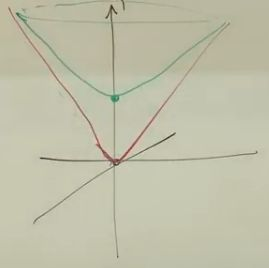
\includegraphics[width=\textwidth]{cosmo-3-hyperboloid}
	\end{subfigure}
	\;
	\begin{subfigure}[t]{0.3\textwidth}
		\caption{Stereographic projection. We project points onto plane. Notice asymptotic circle: there are no points outside this. There is a lot of distortion.}
		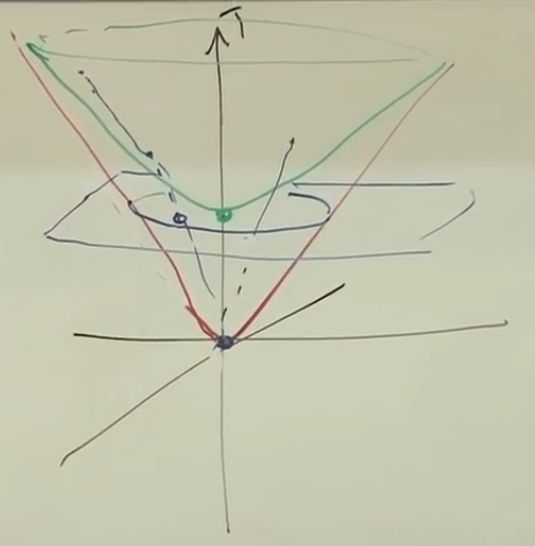
\includegraphics[width=\textwidth]{cosmo-3-hyperboloid-stereographic}
	\end{subfigure}
	\;
	\begin{subfigure}[t]{0.3\textwidth}
		\caption{The angels and devils are supposed to be the same size, and each one sees the same things, and has the same neighbours. There are coordinate transformation that will map one onto the other.}
		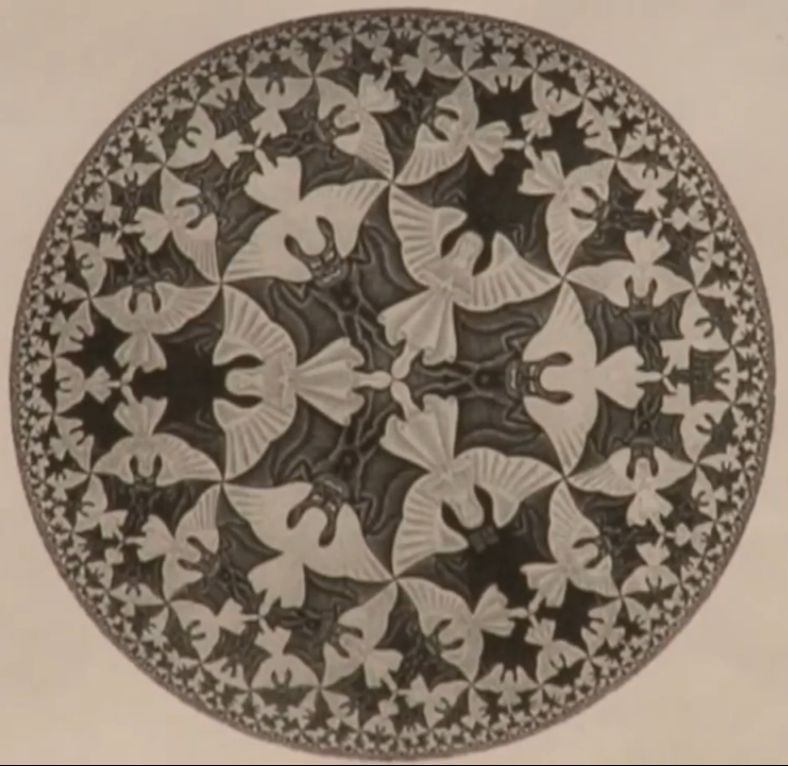
\includegraphics[width=\textwidth]{cosmo3-escher}
	\end{subfigure}
\end{figure}

This geometry has many names. It is also the uniformly negatively curved space.

We can also make the space have a radius other than 1.
\begin{align*}
	ds^2 =& a^2 \big(dr^2 + \sin^2 r d\Omega_{n-1})^2\big) \text{sphere} \\
	ds^2 =& a^2 \big(dr^2 + \sinh^2 r d\Omega_{n-1})^2\big) \text{hyperboloid}
\end{align*}
The smaller $a$, the greater the curvature.

Modern cosmology assumes that the space we live in is one of the three that we have considered.  On scales that we can currently detect, the Universe appears flat--out to 22 billion light years, so we know that the radius must be at least 10 times this side.

Space could also be a torus, a rectangle with opposite sides identified; flat, with periodic boundary conditions. People have looked for evidence of periodicity, but not found any\footnote{This was in response to a question asked at the start of Section \ref{sec:cosmological:thermodynamics}}.
 
 \subsection{Space and Time}
 
 The Minkowski metric is:
 \begin{align*}
 	ds^2 = - dt^2 + dx^2 + dy^2 + dz^2 
 \end{align*}
 
 A light ray (null ray) is $ds^2$=0--$dx=\pm dt$
 
 We will replace $ dx^2 + dy^2 + dz^2 $ with one of the metrics we have discussed, e.g.
  \begin{align*}
 	ds^2 =& - dt^2 + a(t)^2d\Omega_2^2\\
 	D =& a(t) \theta\\
 	V =& \dot{a}\theta\\ 
 	=& \frac{\dot{a}}{a} D \text{, Hubble Law}
 \end{align*}
 
  Space is 2 dimensional, and diameter of space changes with time, $2+1$
  
 Here are our 3 cases of interest:
 \begin{align*}
 	ds^2 =& -dt^2 + a(t)^2 \big( dx^2 + dy^2 + dz^2 \big) \text{, Flat, but scale factor depends on time}\\
 	ds^2 =& - dt^2 + a(t)^2d\Omega_3^2 \text{, spherical, with varying radius}\\
 	ds^2 =& - dt^2 + a(t)^2d\mathcal{H}_3^2 \text{, hyperbolic, with varying radius}
 \end{align*}

We need to investigate how $a$ varies with time. We will need to write down equations from General Relativity. It tuwn out they will agree with the Friedmann equations we derived from Newtonian physics.
\section{Cosmological Thermodynamics}\label{sec:cosmological:thermodynamics}

\begin{quotation}
	The time-time component of Einstein's field equations for general relativity relate energy density to the geometry of space.  Using this energy density, Professor Susskind presents the thermodynamic equation of state which relates the energy density to pressure.  He uses this equation to derive how the density of the universe relates to the scale factor for matter- and radiation-dominated universes, and gives a brief preview of how dark energy affects this analysis.
\end{quotation}

\section{Vacuum energy}

\begin{quotation}
	After a review of the equations of state presented in the last lecture, Professor Susskind derives the density parameter for an energy dominated universe.  He then introduces the concept of vacuum energy, which is represented by the cosmological constant, and is one possible form of dark energy, and describes the characteristics of the universe under various values of the cosmological constant and curvature.
\end{quotation}

\section{Dark matter and allocation of energy density}

\begin{quotation}
	Professor Susskind develops the energy density allocation equation, and describes the historical progress of the effort to find the correct values for the terms in this equation.  This analysis combined with observations of the motion of stars and galaxies led cosmologists to postulate the existence of dark matter.  Observations of luminosity and red-shift have led to the correct solution for today's universe - which is dominated by dark energy.
\end{quotation}

\section{Temperature History of the Universe}

\begin{quotation}
	Professor Susskind examines the temperature history of our universe.  The universe switched from radiation-dominated to matter-dominated when it was about one million times hotter than it is today.  At that time, matter and energy decoupled from each other and the universe became transparent to radiation when it was about one thousand times hotter that it is today.
\end{quotation}

\section{Baryogenesis}

\begin{quotation}
	Professor Susskind opens the lecture with one of the fundamental questions in cosmology: why are there more protons than anti-protons in the universe today? The answer lies in theory of baryogenesis in the very early universe.  This theory leads to the Sakharov conditions, and the fact that the only general symmetry requirement under all conditions is complete charge-parity-time (CPT) symmetry.
	
	Professor Susskind then introduces the concept of inflation in the early universe.  He derives the basic equations of motion for inflation by starting with the equations for a falling particle in a gravitational field and a viscous fluid
\end{quotation}

\section{Inflation}

\begin{quotation}
	
	
	Professor Susskind introduces the theory of cosmological inflation under which the early universe underwent an exponential expansion during which it doubled in size every 10-32 seconds and expanded by at least a factor of $e^{90}$.  This all occurred prior to the Big Bang and during this period the universe cooled very rapidly and was essentially empty.  In the early phase of this rapid expansion, the universe was hot enough that magnetic monopoles were formed.  However these were the only particles formed.  The rest of the energy of the universe was contained in the potential energy of the inflaton field, and it wasn't until the Big Bang that this potential energy was converted into the particles that form the matter that makes up the galaxies in the universe today.
	
	This theory of rapid expansion explains the lack of observed magnetic monopoles and the uniformity of the cosmic microwave background radiation.  The rapid expansion dispersed the monopoles, smoothed out the distribution of photons, and also flattened space itself.
	
\end{quotation}

\section{Inhomogeneities and quantum fluctuations}

\begin{quotation}
Professor Susskind describes the theory whereby inhomogeneities in the universe were caused by quantum fluctuations in the early universe.  He begins with the mathematical equations of a damped harmonic oscillator, and relates that simple system to a dissipative inflation field with spatial dependencies.  The quantum fluctuations in the zero point energy states of this field lead to inhomogeneities in the universe.  These inhomogeneities explain both the small variations in the cosmic microwave background, as well as the formation of galaxies from regions of high energy density.
\end{quotation}

% glossary: may need command makeglossaries.exe cosmology
\printglossaries

\bibliographystyle{unsrt}
\addcontentsline{toc}{section}{Bibliography}
\raggedright
\bibliography{tm}

\end{document}
